%
\documentclass{chi-ext}
% Please be sure that you have the dependencies (i.e., additional LaTeX packages) to compile this example.
% See http://personales.upv.es/luileito/chiext/

%% EXAMPLE BEGIN -- HOW TO OVERRIDE THE DEFAULT COPYRIGHT STRIP -- (July 22, 2013 - Paul Baumann)
\copyrightinfo{Copyright {2014} held by Cefn Hoile. Rights Licensed to ACM}
%% EXAMPLE END -- HOW TO OVERRIDE THE DEFAULT COPYRIGHT STRIP -- (July 22, 2013 - Paul Baumann)

\title{Firmware: The Missing Blueprint}

% Notice how author names are alternately typesetted to appear ordered in 2-column format;
% i.e., the first 4 autors on the first column and the other 4 auhors on the second column.
% Actually, it's up to you to strictly adhere to this author notation.
\author{
  \alignauthor{
        \textbf{Cefn Hoile}\\
        \affaddr{Highwire DTC}\\
        \affaddr{Lancaster University}\\
        \email{c.hoile@lancaster.ac.uk}
  }
  \vspace{2em}
  \begin{figure}
  \centering
  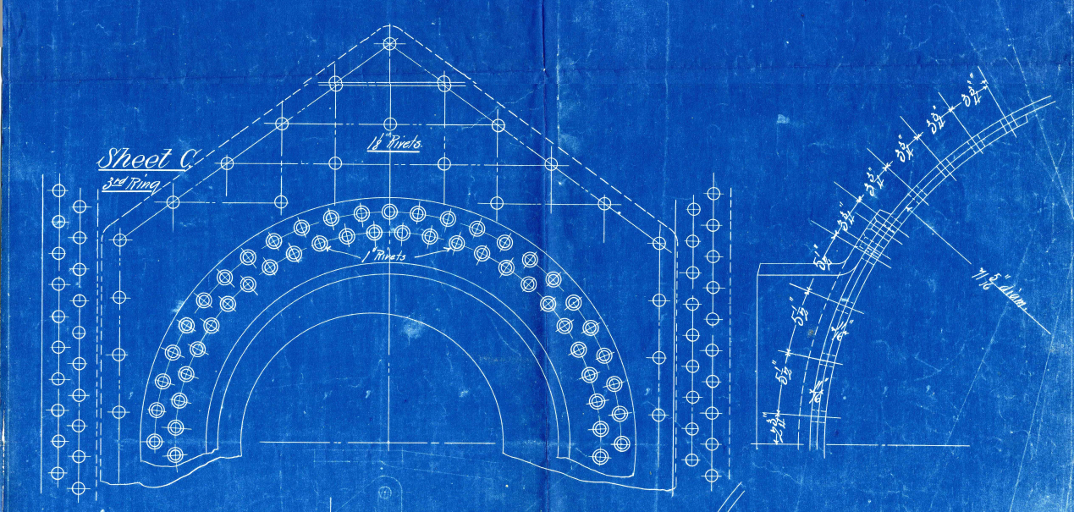
\includegraphics[width=260]{blueprint.jpg}
  \end{figure}
  \vspace{2em}
}

% Paper metadata (use plain text, for PDF inclusion and later re-using, if desired)
\def\plaintitle{CHI LaTeX Extended Abstracts Template}
\def\plainauthor{Luis A. Leiva}
\def\plainkeywords{Guides, instructions, author's kit, conference publications}
\def\plaingeneralterms{Documentation, Standardization}

\hypersetup{
  % Your metadata go here
  pdftitle={\plaintitle},
  pdfauthor={\plainauthor},  
  pdfkeywords={\plainkeywords},
  pdfsubject={\plaingeneralterms},
  % Quick access to color overriding:
  %citecolor=black,
  %linkcolor=black,
  %menucolor=black,
  %urlcolor=black,
}

\usepackage{verbatim}
\usepackage{graphicx}   % for EPS use the graphics package instead
\usepackage{balance}    % useful for balancing the last columns
\usepackage{bibspacing} % save vertical space in references
\renewcommand{\sfdefault}{phv} % Arial
\fontsize{8.5}{10}
\begin{document}

\marginpar{
\begin{figure}
  \begin{center}
  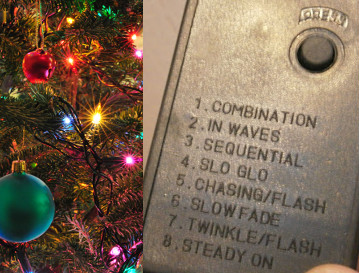
\includegraphics[width=\marginparwidth]{xmas.jpg}
  \caption{Flashing Tree Lights}
  \label{fig:marginparsample}
  \end{center}  
\end{figure}
\vspace{1em}
}

\marginpar{
\begin{figure}
  \begin{center}
  \includegraphics[width=\marginparwidth]{microwave.jpg}
  \caption{Domestic Microwave}
  \label{fig:marginparsample}
  \end{center}  
\end{figure}
\vspace{1em}
}

\marginpar{
\begin{figure}
  \begin{center}
  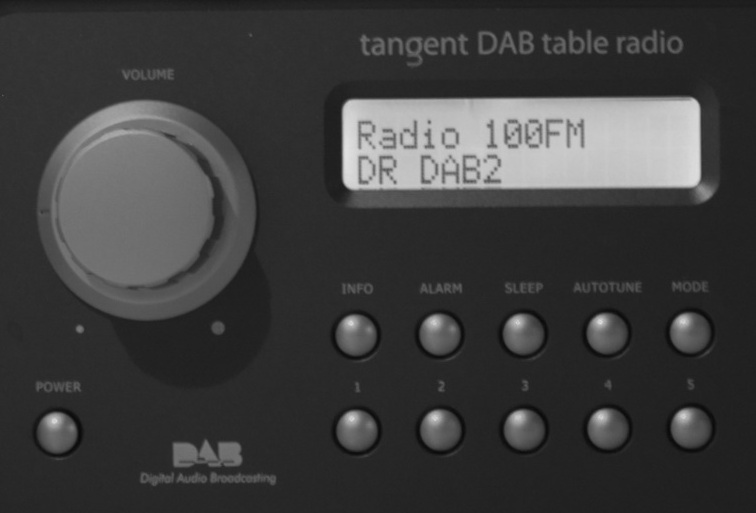
\includegraphics[width=\marginparwidth]{radio.jpg}
  \caption{Digital Radio}
  \label{fig:marginparsample}
  \end{center}  
\end{figure}
\vspace{1em}
}

\maketitle

\begin{abstract}
For a digitally-controlled product, its programmed behaviour, authored through firmware,  will heavily influence user experience. We contrast three caricatures of practice in  which product configurations are either \emph{discovered}, \emph{decided} or \emph{designed}, and focus on the role of  reflective practice, through sketching and boundary objects as a foundation for design. On this analysis, established practice in firmware engineering for selecting programmed behaviour does not satisfy the criteria for being reflectively designed. We examine what obstacles exist to applying reflective practices when selecting the \emph{behaviour} of products, and propose a programme to identify artefacts and processes which can facilitate this work.
\end{abstract}

\begin{comment}
\vspace{1mm}
\noindent
{\bf Categories and Subject Descriptors:} D.2.1 {Requirements/Specification}: {Elicitation Methods

\vspace{1mm}
\noindent
{\bf General Terms:} Enter your choices of the 16 terms.

\vspace{1mm}
\noindent
{\bf Keywords:} Enter your choices.
 \end{comment}

\keywords{Firmware, Microcontrollers, Product Design, Design Interactions, Sketching, Boundary Objects}

\category{D.2.1}{Requirements/Specifications}{Elicitation} 
 
\terms{Design, Human Factors, Experimentation

% =============================================================================
\section{Introduction}
% =============================================================================

An inclusive definition of design, offered by Feng and Feenberg [], is "a process of consciously shaping an artifact to adapt it to specific goals and environments". 

However, not all shaping practices adopt a designerly [] world-view. Some are close to a scientific method, where choices are \emph{discovered}, deducing them from facts. For example, a material's physical properties can eliminate it from consideration, or experiments can recommend employing a particular approach over an alternative. Other practices map a space of solutions on many dimensions of assessment, so a configuration can be \emph{decided} based on an explicit or implicit scheme of values and preferences [].

\marginpar{
\begin{figure}
  \begin{center}
  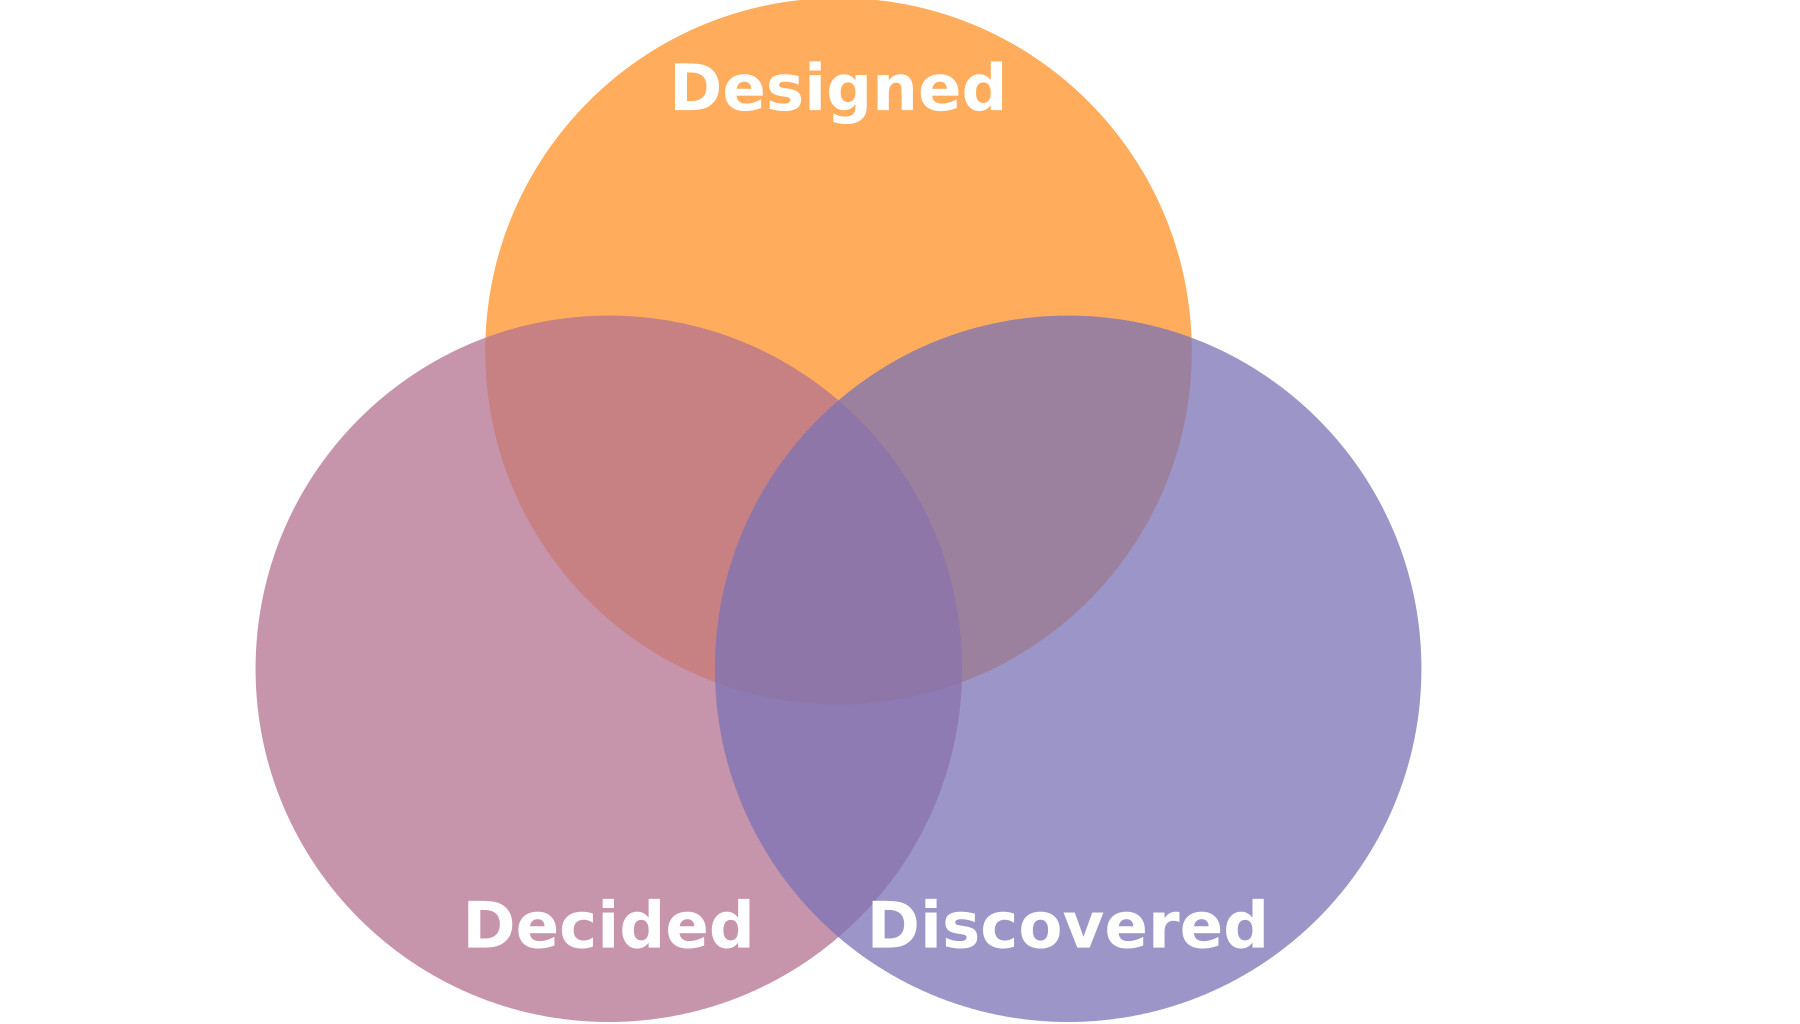
\includegraphics[width=\marginparwidth]{disciplines.jpg}
  \caption{Configuration Choice}
  \label{fig:marginparsample}
  \end{center}  
\end{figure}
}

So, how is designing distinct from discovering or decision-making? In this paper, we employ a definition of design, following Fallman[] and Louridas[], where the phrase \emph{designed} is reserved for artifact shaping which is arrived at through reflective processes [Schon]. \emph{Designed} preferences are neither \emph{discovered} through evidence gathering, nor \emph{decided} through systematic analysis of a space of configurations. Instead, a designer engages in a "conversation with materials" [Schon], a dynamic process in which "the materials [designers] use begin to 'talk back'". [Ozenc et al]

Our position resonates strongly with Fallman's [], that sketching is "the archetypal activity of the design approach". However, if there are no candidate practices within firmware engineering which parallel \emph{sketching}, and if reflective techniques are central to value-creation in all design disciplines, we may ask whether product firmware is actually designed at all?

This paper explores candidate materials to support reflective design within firmware engineering, considering approaches used within the field and comparing them to those from established design disciplines. We offer reasons why familiar approaches cannot be trivially transferred to firmware engineering. We then propose a number of candidates for reflective materials which may be used effectively in firmware design and describe a programme of experimentation to discover how those tools and approaches may sustain the co-design of product firmware.

% =============================================================================
\section{Sketching, Immateriality, Processuality}
% =============================================================================

Designers rely on sketching because it �supports cognition in ways that lead to creativity�, including �re-interpretive cycles of idea generation�. \cite{Craft}, rough out ideas�, then �critique what they have done", using it as a mechanism of reflection \cite{Ozenc}.  

Familiar techniques allow graphic artifacts or physical products to be represented but capturing product \emph{firmware} on the page of a sketchbook presents problems, since it is both immaterial \cite{Ozenc} and processual \cite{Bratteteig}. Since firmware is immaterial, there is no trivial two-dimensional projection of its code which a designer can be expected to author or interpret. Since it is processual, product behaviour is by nature determined by circumstance and history, meaning that any static representations deliver only a partial view of the design. 

However when designing interactive systems, "a designer has not had enough feedback to know if this is the design they want� \cite{Ozenc}. 

Sketches also act as a record of the many alternatives considered, and facilitate sharing to establish collaboration and consensus \cite{VanDerLugt}. 


% =============================================================================
\section{Firmware Engineering}
% =============================================================================

Reports on established practice suggests the early phases of behaviour design for digitally-controlled products are centred on representations primarily accessible to programmers  [Petre 2013]. Development begins with a software requirements document, and proceeds through software modelling constructs and program code until a single prototype implementation can be deployed [Ganssle 2000]. During these phases many choices are made which will impact on the interaction design embodied by the product. However, it is only after a working prototype is deployed that feedback is anticipated from end-users on the behaviour design choices already made [Punkka 2005, van der Helm 2008].

By contrast with other design disciplines, this practice raises the concern that behaviour design decisions for digitally-controlled products could be made overwhelmingly by software engineers on behalf of users, exploring few alternatives, and in isolation from user design contributions (Norman 2006). Assuming that a prototype is needed to sustain engagement, user feedback is only possible late in the firmware design process and inherently centres around approving or critiquing a single behaviour design configuration. Critiques of firmware design [Norman 2002, 2010, Thimbleby 2007, Ganssle 2000) suggest that limitations of existing practice has a direct impact on the quality of products in the marketplace.

\marginpar{
\begin{figure}
  \begin{center}
  \includegraphics[width=\marginparwidth]{bikelight.jpg}
  \caption{Bikelights are computers too}
  \label{fig:marginparsample}
  \end{center}  
\end{figure}
\vspace{1em}
}

Entrenched problems in the industry are illustrated well by Cateye�s SL110 Loop Orbit bikelights, (Amazon 2013) which prompted the following customer report "The back light turns off after 1 minute! I can not use the set when cycling at night as it is unsafe." A bike light unsuitable for use at night fails spectacularly to meet its design brief. The product manual reveals the secret - "Deactivate...�Try Me�...mode (by pressing and holding the light until it flashes quickly and shuts off)".

% =============================================================================
\section{Projection, Immateriality and Processuality}
% =============================================================================



% =============================================================================
\section{Blueprints, Patterns, Collaboration and Co-design}
% =============================================================================

Many participants in a physical design process lack the skills needed to actually materialise the product. Nevertheless, sketches, blueprints and models can serve to catalyse knowledge exchange between a wide range of stakeholders, helping to integrate clients' experience of the market and users' experience of the domain from a very early stage in the design process of a physical product.

Blueprints of physical designs capture implementation commitments, guiding and constraining a specialist production process. However, they also stimulate and facilitate engagement with others without demanding they themselves have the skills to materialise the design. By contrast, in a firmware design process, the representations which characterise implementation commitments for code are accessible principally to programmers - those skilled in materialising digital behaviours - and can not effectively catalyse knowledge exchange with others. By excluding key stakeholders until working systems are ready to be tested, this restricts the design contributions they can make, and limits the potential for design thinking. 

Blueprints delivery downstream

Multiplicity and Engagement

Patterns engagement upstream

% =============================================================================
\section{Boundary Objects and Bricolage}
% =============================================================================

Design disciplines such as product design and architecture have mature techniques to engage end-users early in the design process, whilst stimulating and recording multiple alternative choices for downstream implementation (Cross 2006)(Eriksen 2008). These techniques range from unstructured, informal practices such as brainstorming (Gerber and Carroll 2012), (Cruickshank and Evans 2012) (van der Lugt 2002), sketching (Arvola and Artman 2007), (Craft and Cairns 2009), and low-fidelity prototypes (Muller 1999,Gerber and Carroll 2012, Rice et al 2012, Rhinow et al 2012) through to more formal structured practices such as method cards (Lockton et al 2010, Biskjaer et al 2010, Sangiorgi and Clark 2004) and blueprints (Nystrom 2007, Hansen et al 2012). These boundary objects (Star and Greisemer 1989) factor significantly in user-led design processes, helping �design intent� to be communicated, and facilitating reflection (Schon 1992). The techniques act to surface, record and resolve concerns in design choices before significant investments are made fabricating prototypes or materialising the final design. 


 and bricolage [Levi-Strauss], building on design theorist's claims that  [Fallman] and that "design in all its guises is a form of bricolage"[Louridas].


% =============================================================================
\section{Wizard of Oz and Visual Programming}
% =============================================================================



\marginpar{
\begin{figure}
  \begin{center}
  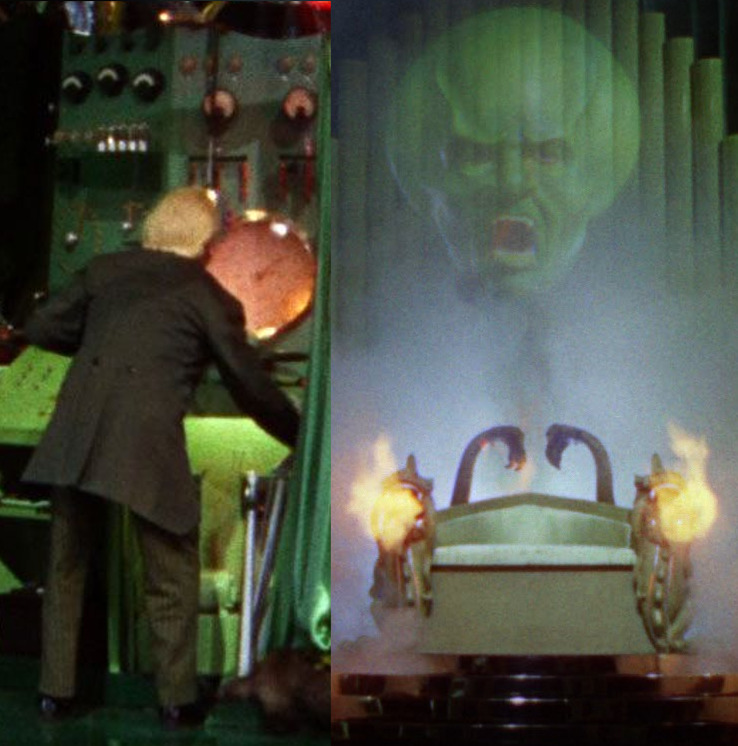
\includegraphics[width=\marginparwidth]{wizard_of_oz.jpg}
  \caption{The Wizard Of Oz}
  \label{fig:marginparsample}
  \end{center}  
\end{figure}
}

\marginpar{
\begin{figure}
  \begin{center}
  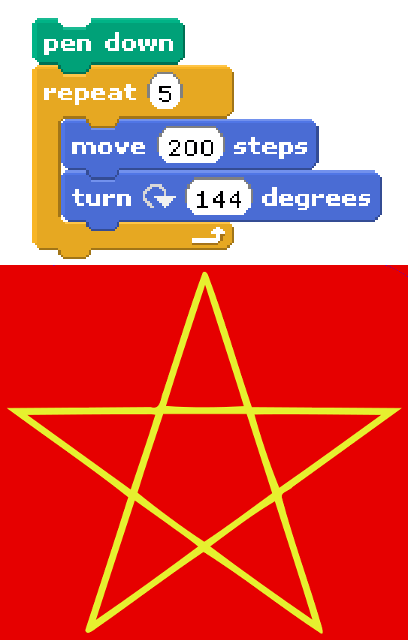
\includegraphics[width=\marginparwidth]{scratch.png}
  \caption{Program in Scratch}
  \label{fig:marginparsample}
  \end{center}  
\end{figure}
}

\begin{comment}
\begin{figure}
  \centering
  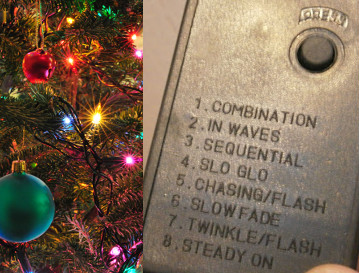
\includegraphics[width=\linewidth]{sample.jpg}
  \caption{Flashing Christmas Lights}
  \label{fig:sample}
\end{figure}
\end{comment}

We outline the preferred features by analogy with effective tools from other disciplines, and we detail a program of future co-design experimentation which we hope will allow us to explore and validate candidate representations.


% =============================================================================
\section{Conclusion}
% =============================================================================

Critiques levelled at mainstream interaction design suggest that practice should change.

\section{Acknowledgements}
NYU Dead Media Archive [Blueprint image]
Creative Commons imagery [Flickr accounts clagnut,]
SarahMumOf3 for Xmas Light controller


\section{References format}
References must be the same font size as other body text.
% REFERENCES FORMAT
% References must be the same font size as other body text.

\balance
\bibliographystyle{acm-sigchi}
\bibliography{sample}

\end{document}
